\documentclass{tufte-book}

\usepackage{ulem}
\usepackage{amsmath}
\usepackage{amsthm}
\usepackage{amsfonts}

\hypersetup{colorlinks}% uncomment this line if you prefer colored hyperlinks (e.g., for onscreen viewing)

%%
% Book metadata
\title{Problem Sets Vol. II}
\author[Alex Cooper]{Alex Cooper}
\publisher{adrcooper.com}

%%
% If they're installed, use Bergamo and Chantilly from www.fontsite.com.
% They're clones of Bembo and Gill Sans, respectively.
\IfFileExists{bergamo.sty}{\usepackage[osf]{bergamo}}{}% Bembo
\IfFileExists{chantill.sty}{\usepackage{chantill}}{}% Gill Sans

\usepackage{microtype}

%%
% For nicely typeset tabular material
\usepackage{booktabs}

%%
% For graphics / images
\usepackage{graphicx}
\setkeys{Gin}{width=\linewidth,totalheight=\textheight,keepaspectratio}
\graphicspath{{graphics/}}

\usepackage{array}
\providecommand{\tabularnewline}{\\}

% The fancyvrb package lets us customize the formatting of verbatim
% environments.  We use a slightly smaller font.
\usepackage{fancyvrb}
\fvset{fontsize=\normalsize}

%%
% Prints argument within hanging parentheses (i.e., parentheses that take
% up no horizontal space).  Useful in tabular environments.
\newcommand{\hangp}[1]{\makebox[0pt][r]{(}#1\makebox[0pt][l]{)}}

%%
% Prints an asterisk that takes up no horizontal space.
% Useful in tabular environments.
\newcommand{\hangstar}{\makebox[0pt][l]{*}}

%%
% Prints a trailing space in a smart way.
\usepackage{xspace}

%%
% Some shortcuts for Tufte's book titles.  The lowercase commands will
% produce the initials of the book title in italics.  The all-caps commands
% will print out the full title of the book in italics.
\newcommand{\vdqi}{\textit{VDQI}\xspace}
\newcommand{\ei}{\textit{EI}\xspace}
\newcommand{\ve}{\textit{VE}\xspace}
\newcommand{\be}{\textit{BE}\xspace}
\newcommand{\VDQI}{\textit{The Visual Display of Quantitative Information}\xspace}
\newcommand{\EI}{\textit{Envisioning Information}\xspace}
\newcommand{\VE}{\textit{Visual Explanations}\xspace}
\newcommand{\BE}{\textit{Beautiful Evidence}\xspace}

\newcommand{\TL}{Tufte-\LaTeX\xspace}

% Prints the month name (e.g., January) and the year (e.g., 2008)
\newcommand{\monthyear}{%
  \ifcase\month\or January\or February\or March\or April\or May\or June\or
  July\or August\or September\or October\or November\or
  December\fi\space\number\year
}


% Prints an epigraph and speaker in sans serif, all-caps type.
\newcommand{\openepigraph}[2]{%
  %\sffamily\fontsize{14}{16}\selectfont
  \begin{fullwidth}
  \sffamily\large
  \begin{doublespace}
  \noindent\allcaps{#1}\\% epigraph
  \noindent\allcaps{#2}% author
  \end{doublespace}
  \end{fullwidth}
}

% Inserts a blank page
\newcommand{\blankpage}{\newpage\hbox{}\thispagestyle{empty}\newpage}

\usepackage{units}

% Typesets the font size, leading, and measure in the form of 10/12x26 pc.
\newcommand{\measure}[3]{#1/#2$\times$\unit[#3]{pc}}

% Macros for typesetting the documentation
\newcommand{\hlred}[1]{\textcolor{Maroon}{#1}}% prints in red
\newcommand{\hangleft}[1]{\makebox[0pt][r]{#1}}
\newcommand{\hairsp}{\hspace{1pt}}% hair space
\newcommand{\hquad}{\hskip0.5em\relax}% half quad space
\newcommand{\TODO}{\textcolor{red}{\bf TODO!}\xspace}
\newcommand{\ie}{\textit{i.\hairsp{}e.}\xspace}
\newcommand{\eg}{\textit{e.\hairsp{}g.}\xspace}
\newcommand{\na}{\quad--}% used in tables for N/A cells
\providecommand{\XeLaTeX}{X\lower.5ex\hbox{\kern-0.15em\reflectbox{E}}\kern-0.1em\LaTeX}
\newcommand{\tXeLaTeX}{\XeLaTeX\index{XeLaTeX@\protect\XeLaTeX}}
% \index{\texttt{\textbackslash xyz}@\hangleft{\texttt{\textbackslash}}\texttt{xyz}}
\newcommand{\tuftebs}{\symbol{'134}}% a backslash in tt type in OT1/T1
\newcommand{\doccmdnoindex}[2][]{\texttt{\tuftebs#2}}% command name -- adds backslash automatically (and doesn't add cmd to the index)
\newcommand{\doccmddef}[2][]{%
  \hlred{\texttt{\tuftebs#2}}\label{cmd:#2}%
  \ifthenelse{\isempty{#1}}%
    {% add the command to the index
      \index{#2 command@\protect\hangleft{\texttt{\tuftebs}}\texttt{#2}}% command name
    }%
    {% add the command and package to the index
      \index{#2 command@\protect\hangleft{\texttt{\tuftebs}}\texttt{#2} (\texttt{#1} package)}% command name
      \index{#1 package@\texttt{#1} package}\index{packages!#1@\texttt{#1}}% package name
    }%
}% command name -- adds backslash automatically
\newcommand{\doccmd}[2][]{%
  \texttt{\tuftebs#2}%
  \ifthenelse{\isempty{#1}}%
    {% add the command to the index
      \index{#2 command@\protect\hangleft{\texttt{\tuftebs}}\texttt{#2}}% command name
    }%
    {% add the command and package to the index
      \index{#2 command@\protect\hangleft{\texttt{\tuftebs}}\texttt{#2} (\texttt{#1} package)}% command name
      \index{#1 package@\texttt{#1} package}\index{packages!#1@\texttt{#1}}% package name
    }%
}% command name -- adds backslash automatically
\newcommand{\docopt}[1]{\ensuremath{\langle}\textrm{\textit{#1}}\ensuremath{\rangle}}% optional command argument
\newcommand{\docarg}[1]{\textrm{\textit{#1}}}% (required) command argument
\newenvironment{docspec}{\begin{quotation}\ttfamily\parskip0pt\parindent0pt\ignorespaces}{\end{quotation}}% command specification environment
\newcommand{\docenv}[1]{\texttt{#1}\index{#1 environment@\texttt{#1} environment}\index{environments!#1@\texttt{#1}}}% environment name
\newcommand{\docenvdef}[1]{\hlred{\texttt{#1}}\label{env:#1}\index{#1 environment@\texttt{#1} environment}\index{environments!#1@\texttt{#1}}}% environment name
\newcommand{\docpkg}[1]{\texttt{#1}\index{#1 package@\texttt{#1} package}\index{packages!#1@\texttt{#1}}}% package name
\newcommand{\doccls}[1]{\texttt{#1}}% document class name
\newcommand{\docclsopt}[1]{\texttt{#1}\index{#1 class option@\texttt{#1} class option}\index{class options!#1@\texttt{#1}}}% document class option name
\newcommand{\docclsoptdef}[1]{\hlred{\texttt{#1}}\label{clsopt:#1}\index{#1 class option@\texttt{#1} class option}\index{class options!#1@\texttt{#1}}}% document class option name defined
\newcommand{\docmsg}[2]{\bigskip\begin{fullwidth}\noindent\ttfamily#1\end{fullwidth}\medskip\par\noindent#2}
\newcommand{\docfilehook}[2]{\texttt{#1}\index{file hooks!#2}\index{#1@\texttt{#1}}}
\newcommand{\doccounter}[1]{\texttt{#1}\index{#1 counter@\texttt{#1} counter}}

% Generates the index
\usepackage{makeidx}
\makeindex

\begin{document}

\frontmatter

\maketitle

\mainmatter

\newpage\section{Problem Set \textnumero 1}

\begin{enumerate}
  \item Nouns are words that describe things, objects, or people. \underline{Underline} the nouns in the following sentences.
  \begin{enumerate}
    \item My dog can juggle three watermelons while riding a unicycle.
    \item A grumpy ghost in my closet keeps asking for a sandwich.
    \item The school bus is powered by a giant sneeze from Puff, a friendly dragon.
    \item For breakfast, I ate a pancake shaped like a stegosaurus.
  \end{enumerate}

  \item \bigskip\marginnote{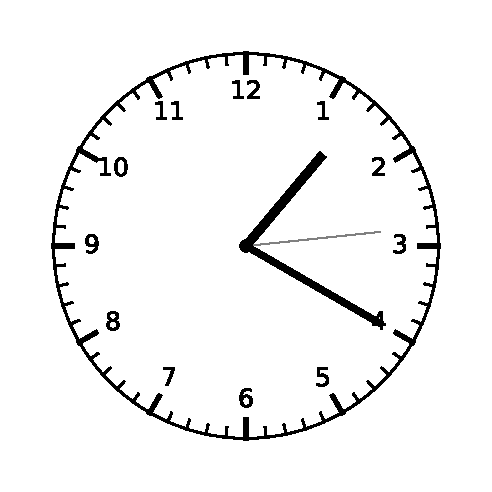
\includegraphics[width=0.5\textwidth]{maths/fig/clock_0120.pdf}} 
  What's the time? \dotfill\bigskip\par\dotfill\bigskip.
  
  \item Farmer Giles grew one thousand, nine hundred and ninety-eight singing potatoes.
  A flock of very hungry seagulls ate six hundred and eighty-nine of them.
  How many singing potatoes are left?\bigskip\par
Number sentence: \dotfill\bigskip\par
Answer: There are
\dotfill\bigskip\par\mbox{}\dotfill\bigskip\par\mbox{}\dotfill\bigskip\par\dotfill\bigskip
 singing potatoes left.

  \item Note on the Venn diagram where each of the following things belong:
  parakeets, rockets, ostriches, sugar gliders.\par
  {\centering 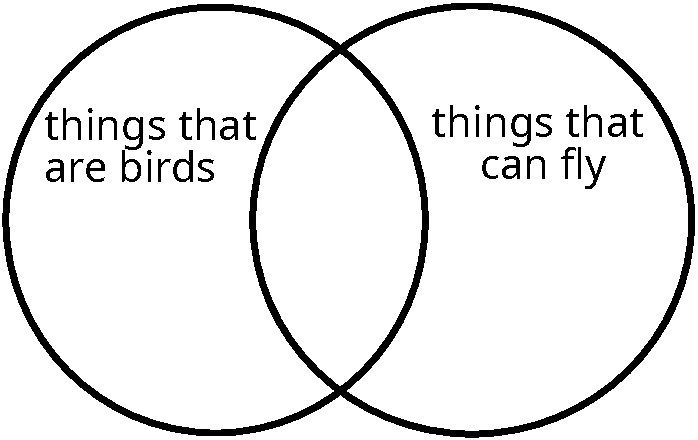
\includegraphics[width=0.8\textwidth]{maths/fig/venn_birds_fly.pdf}}

\end{enumerate}

\newpage\section{Problem Set \textnumero 2}

\begin{enumerate}
  \item Find ten nouns in this picture of a classroom.\bigskip
  \begin{marginfigure}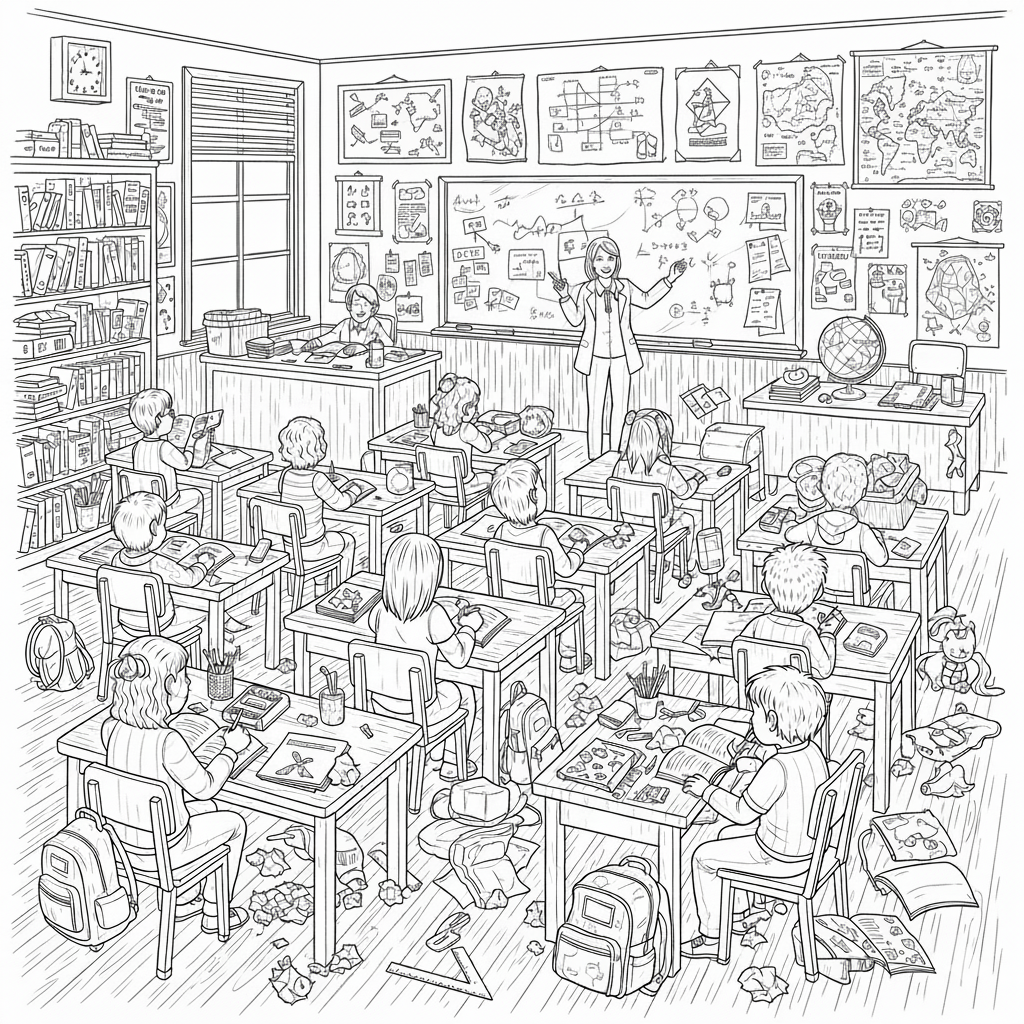
\includegraphics[width=\textwidth]{grammar/classroom.png}\end{marginfigure}
\begin{multicols}{2}
  \begin{enumerate}
    \item \dotfill\bigskip
    \item \dotfill\bigskip
    \item \dotfill\bigskip
    \item \dotfill\bigskip
    \item \dotfill
    \item \dotfill\bigskip
    \item \dotfill\bigskip
    \item \dotfill\bigskip
    \item \dotfill\bigskip
    \item \dotfill\bigskip
  \end{enumerate}
\end{multicols}

\item A grumpy gargoyle found seven hundred and sixty-five shiny bottle caps.
He then found two hundred and thirty-six more.
How many bottle caps does the gargoyle have in total?\bigskip\par
Number sentence: \dotfill\bigskip\par
Answer: The gargoyle has 
\dotfill\medskip\par\mbox{}\dotfill\medskip\par\mbox{}\dotfill\bigskip
 bottle caps in total.

\item The time is \dotfill\bigskip\par\dotfill\bigskip.
\begin{marginfigure}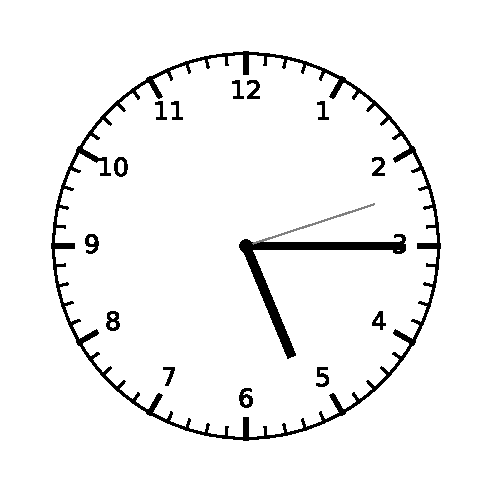
\includegraphics[width=\textwidth]{maths/fig/clock_0515.pdf}\end{marginfigure}

\item On the Venn diagram, note where each of the following things belong:
growl, speaking, snort, burp, giggle, meow.

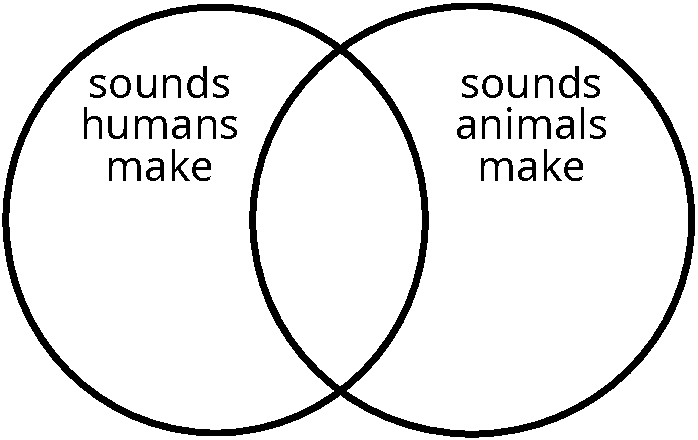
\includegraphics[width=0.9\textwidth]{maths/fig/venn_sounds.pdf}

\end{enumerate}

\clearpage\section{Problem Set \textnumero 3}

\begin{enumerate}
  \item Complete each sentence by filling in each blank with a \textbf{noun}.
  \begin{enumerate}
    \bigskip
    \item Princess Fluffybutt ate three\dotfill.\bigskip
    \item Professor Bumble wrote a \dotfill.\bigskip
    \item The \dotfill was chasing the \dotfill.\bigskip
    \item The sneaky cat broke the \dotfill.\bigskip
    \item The treasure chest contained \dotfill.\bigskip
  \end{enumerate}

  \item Princess Penelope likes animals. 
  She has eight unicorns, six penguins, twelve cats, a guinea pig, three puppies,
  one hundred and three mice, and a sugar glider.
  How many pets does Princess Penelope have in total?\bigskip\par
  Number sentence: \dotfill\bigskip\par
  Answer: Princess Penelope has \dotfill\bigskip\par\dotfill\bigskip pets.

  \item The time is \dotfill\bigskip\par\dotfill\bigskip.
  \begin{marginfigure}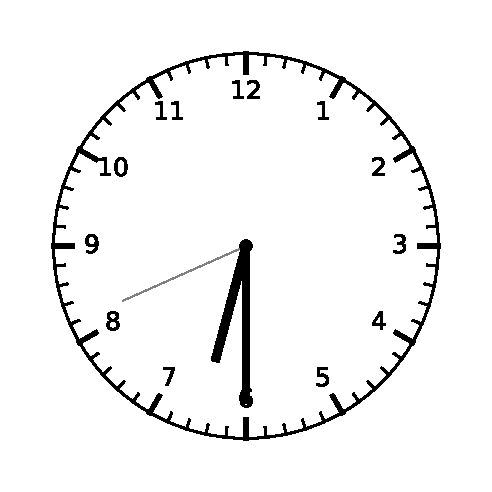
\includegraphics[width=\textwidth]{maths/fig/clock_0630.pdf}\end{marginfigure}

  \item The Venn diagram shows the contents of two sets, $A$ and $B$.
  \begin{marginfigure}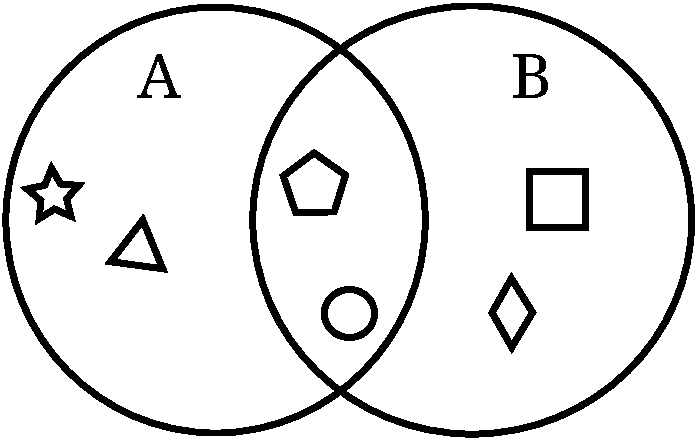
\includegraphics[width=\textwidth]{maths/fig/venn_sets.pdf}\end{marginfigure}
  What are the elements:
  \begin{enumerate}
    \item in set $A$:\dotfill\bigskip
    \item in set $B$:\dotfill\bigskip
    \item \emph{both} in set $A$ and in set $B$:\dotfill\bigskip
    \item in set {A} \emph{but not} in set {B}:\dotfill\bigskip
  \end{enumerate}

\end{enumerate}

\clearpage\section{Problem Set \textnumero 4}

\begin{enumerate}
  \item A \textbf{proper noun} starts with a capital letter and names a particular person, place, season, etc. Other nouns are called \textbf{common nouns}.
  \underline{Underline} the proper nouns and \uwave{squiggle} under the common nouns in these sentences.
  \begin{enumerate}
    \item \underline{Spot} likes to chase \uwave{mice} in the \uwave{garden} during \underline{Spring}.
    \item Miss Fluffybutt is the principal of Fluffybutt Primary School.
    \item The garden is full of flowers in Summer.
    \item My school is located on Stinky Lane.
    \item Several students are having a picnic in the park.
    \item The old teacher is wearing a blue shirt.
    \item The students are having a picnic in the park.
  \end{enumerate}

  \item Princess Penelope had nine thousand, eight hundred and seventy-six soft toys.
  She gave eight thousand, nine hundred and eighty-eight of them away to charity. 
  How many soft toys does Princess Penelope have left?\bigskip\par
  Number sentence: \dotfill\bigskip\par
  Answer: Princess Penelope has \dotfill\bigskip\par\dotfill\bigskip soft toys left.

  \item The time is \dotfill\bigskip\par\dotfill\bigskip.
  \begin{marginfigure}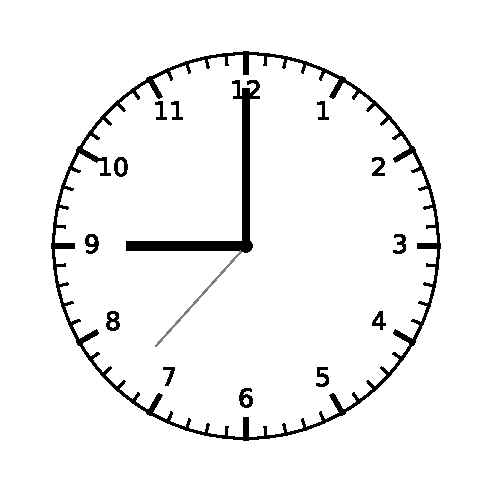
\includegraphics[width=\textwidth]{maths/fig/clock_0900.pdf}\end{marginfigure}

  \item Three boys go to school using a different methods at different speeds.
  The boy who rides his bike goes super fast. Ken does not walk.
  Russ travels at a medium pace. The person who travels slowly is walking.\par
  \begin{tabular}{|l|>{\centering}p{2cm}|>{\centering}p{2cm}|>{\centering}p{2cm}|>{\centering}p{2cm}|>{\centering}p{2cm}|>{\centering}p{2cm}|}
  \hline 
    & \textbf{Walking} & \textbf{Bike} & \textbf{Scooter} & \textbf{Super Fast} & \textbf{Medium} & \textbf{Slowly}\tabularnewline
  \hline 
  \textbf{Bob} &  &  &  &  &  & \tabularnewline
  \hline 
  \textbf{Ken} &  &  &  &  &  & \tabularnewline
  \hline 
  \textbf{Russ} &  &  &  &  &  & \tabularnewline
  \hline 
  \end{tabular}
  \bigskip
  \begin{itemize}
    \item Bob \dotfill\bigskip
    \item Ken \dotfill\bigskip
    \item Russ \dotfill
  \end{itemize}

\end{enumerate}

\clearpage\section{Problem Set \textnumero 5}

\begin{enumerate}
  \item \textbf{Countable nouns} can be counted (e.g. one apple, two apples). \textbf{Uncountable nouns} cannot be counted (e.g. sand, rain, sugar).
  Countable nouns form their plural by adding an "s" to the end of the noun, but uncountable nouns do not have a plural form.
  Next to each noun, write "C" if it is countable, "U" if it is uncountable, or "CU" if it is both.
  \begin{multicols}{3}
  \begin{enumerate}
    \item apple: \dotfill
    \item car: \dotfill
    \item house: \dotfill
    \item wood: \dotfill
    \item water: \dotfill
    \item wine: \dotfill
    \item cheese: \dotfill
    \item pumpkin: \dotfill
    \item bread: \dotfill
    \item milk: \dotfill
    \item sugar: \dotfill
    \item salt: \dotfill
    \item pepper: \dotfill
  \end{enumerate}
  \end{multicols}

  \item \underline{Underline} the proper nouns and \uwave{squiggle} under the common nouns in these sentences.
  \begin{enumerate}
    \item Ben visited Paris with his family.
    \item Ben loves chocolate.
    \item The family ate too much chocolate and had to go for a walk.
    \item Ben and his sister felt very sick and had to go to the doctor.
    \item The doctor gave them some medicine to make them feel better.
    \item Ben's sister threw up all the chocolate she ate.
  \end{enumerate}

  \item The time is \dotfill\bigskip\par\dotfill\bigskip.
  \begin{marginfigure}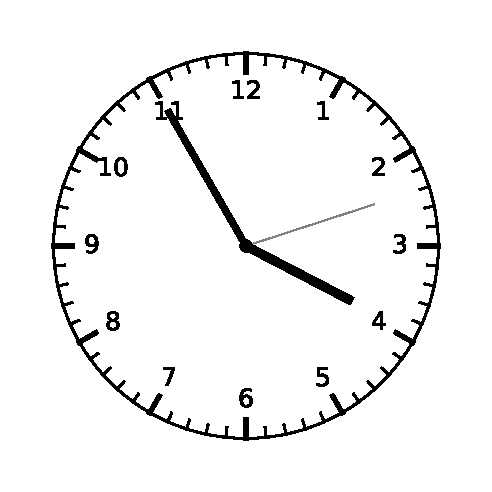
\includegraphics[width=\textwidth]{maths/fig/clock_0355.pdf}\end{marginfigure}

  \item The Venn diagram shows the contents of two sets, $A$ and $B$.
  \begin{marginfigure}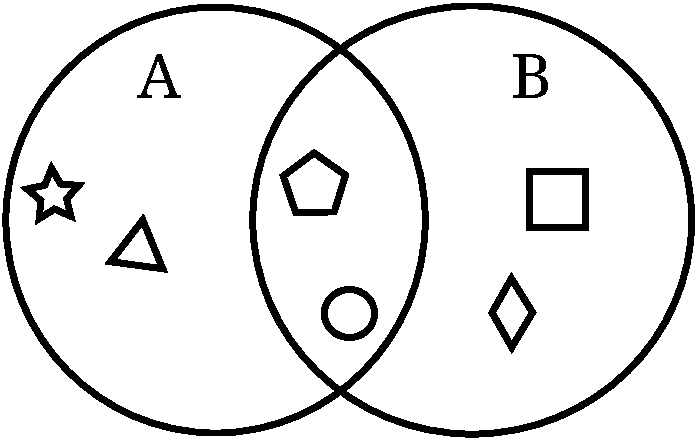
\includegraphics[width=\textwidth]{maths/fig/venn_sets.pdf}\end{marginfigure}
  If $\square$ is in set $S$, mathematicians write $\square \in S$. If $\square$ is not in set $S$, we write $\square \notin S$.
  Fill in the blanks with $\in$ or $\notin$.
  \begin{multicols}{4}
  \begin{enumerate}
    \item $\square$ \dotfill $A$\bigskip
    \item $\square$ \dotfill $B$\bigskip
    \item $\bigcirc$ \dotfill $A$\bigskip
    \item $\bigcirc$ \dotfill $B$\bigskip
    \item $\triangle$ \dotfill $A$\bigskip
    \item $\triangle$ \dotfill $B$\bigskip
  \end{enumerate}
  \end{multicols}
\end{enumerate}

\end{document}
